To solve the constrained optimization problem \eqref{eq:disoTPS_YB_move_alternative_formulation} we proceed by maximizing the overlap while only varying the parameters of one of the three tensors $T^\prime$, $W_1^\prime$ or $W_2^\prime$, treating all other tensors as constant. For example, let us keep $W_1^\prime$ and $W_2^\prime$ fixed and optimize $T^\prime$. We first contract all tensors except $T^\prime$ into an environment $E$ as shown in figure \figref{fig:YB_move_iterate_polar}(b). We can then write the optimization problem as
\begin{equation}
	T^\prime_\text = \underset{T^{\prime\dagger}T = \id}{\argmax} \Re\left\langle\Psi\middle|\Psi^\prime\right\rangle = \underset{T^{\prime\dagger}T = \id}{\argmax}\Re\left\langle T^\prime, E\right\rangle_\text{F} = \underset{T^{\prime\dagger}T = \id}{\argmax}\Re\Tr\left(T^{\prime\dagger}E\right).
\end{equation}
This problem is known as the \textit{orthogonal Procrustes problem} and permits the closed form solution $T^\prime_\text{opt} = UV^\dagger$, where $U$ and $V$ are computed using the SVD $E = USV^\dagger$. For the derivation of this solution see appendix \ref{sec:orthogonal_procrustes_problem}. The tensors $W_1^\prime$ and $W_2^\prime$ can be optimized similarly. The full algorithm is then performed by sweeping over the three tensors, optimizing them iteratively until convergence. Tensor diagrams for the algorithm are shown in figure \figref{fig:YB_move_iterate_polar}. We discuss one iteration of the algorithm in more detail:
\begin{enumerate}
	\item We contract all tensors except $T^\prime$ into an environment $E$ and perform an SVD $E = USV$. The tensor $T^\prime$ is then updated as $T^\prime\leftarrow UV^\dagger$. See figure \figref{fig:YB_move_iterate_polar}(b).
	\item We contract all tensors except $W_1^\prime$ into an environment $E$ and perform an SVD $E = USV$. The tensor $W_1^\prime$ is then updated as $W_1^\prime\leftarrow UV^\dagger$. See figure \figref{fig:YB_move_iterate_polar}(c).
	\item We contract all tensors except $W_2^\prime$ into an environment $E$. The tensor $W_1^\prime$ is then updated as $W_1^\prime\leftarrow E/\left\lVert E\right\rVert$. See figure \figref{fig:YB_move_iterate_polar}(d).
\end{enumerate}
These three steps are repeated until a termination criterion is met, for example until the decrease in error after one iteration is smaller than a given threshold or if a given maximum number of iterations is exceeded.
\todo{Discuss complexity and initialization details!}
\begin{figure}
	\centering
	\subcaptionbox{\label{fig:YB_move_iterate_polar_overlap}}
	{%
		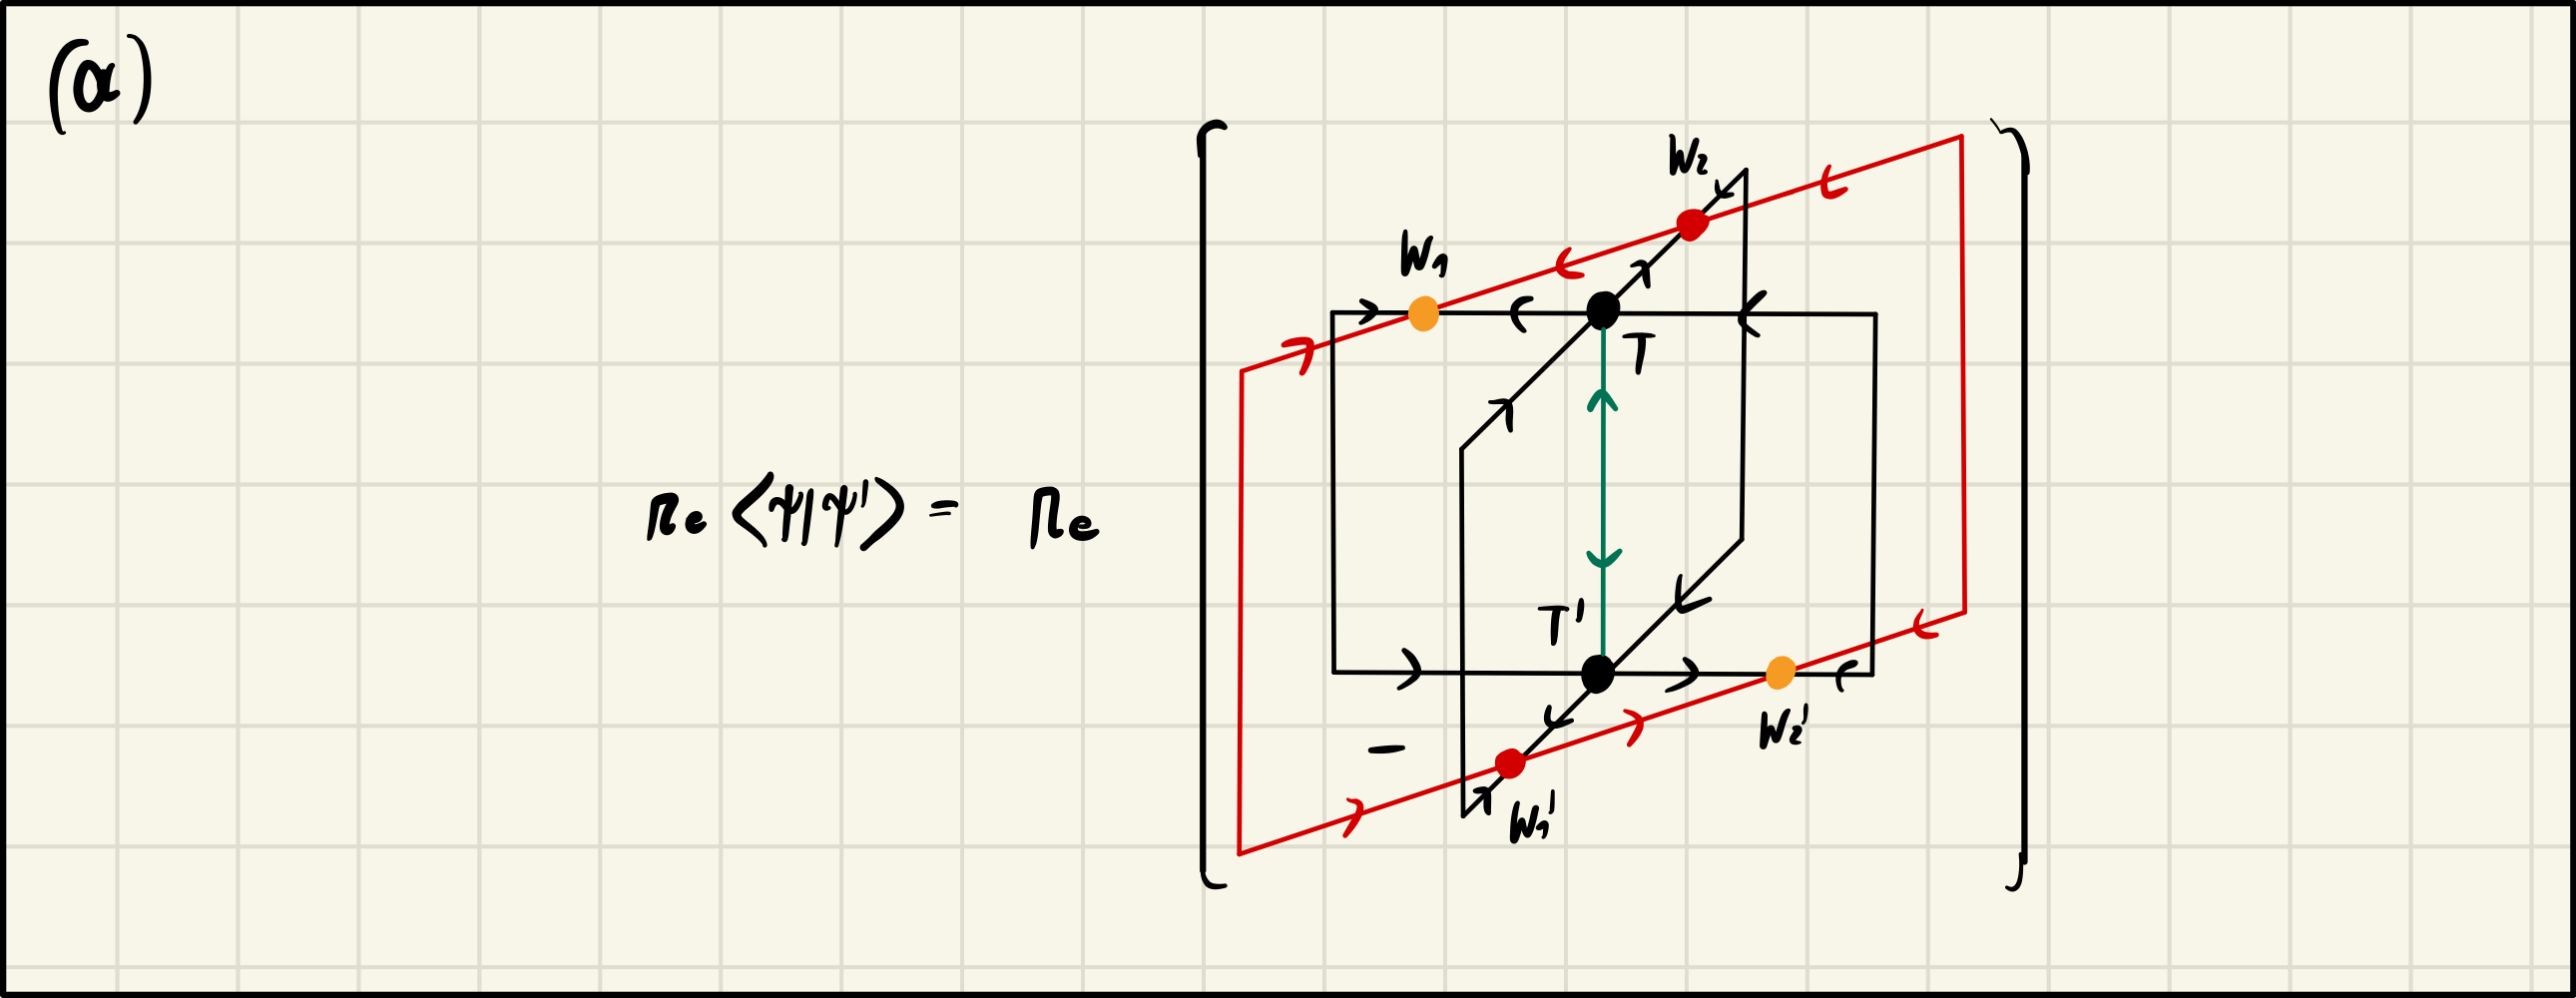
\includegraphics[width=0.6\textwidth]{figures/disoTPS/YB_move_iterate_polar_a.jpeg}
	}
	\subcaptionbox{\label{fig:YB_move_iterate_polar_optimize_W2}}
	{%
		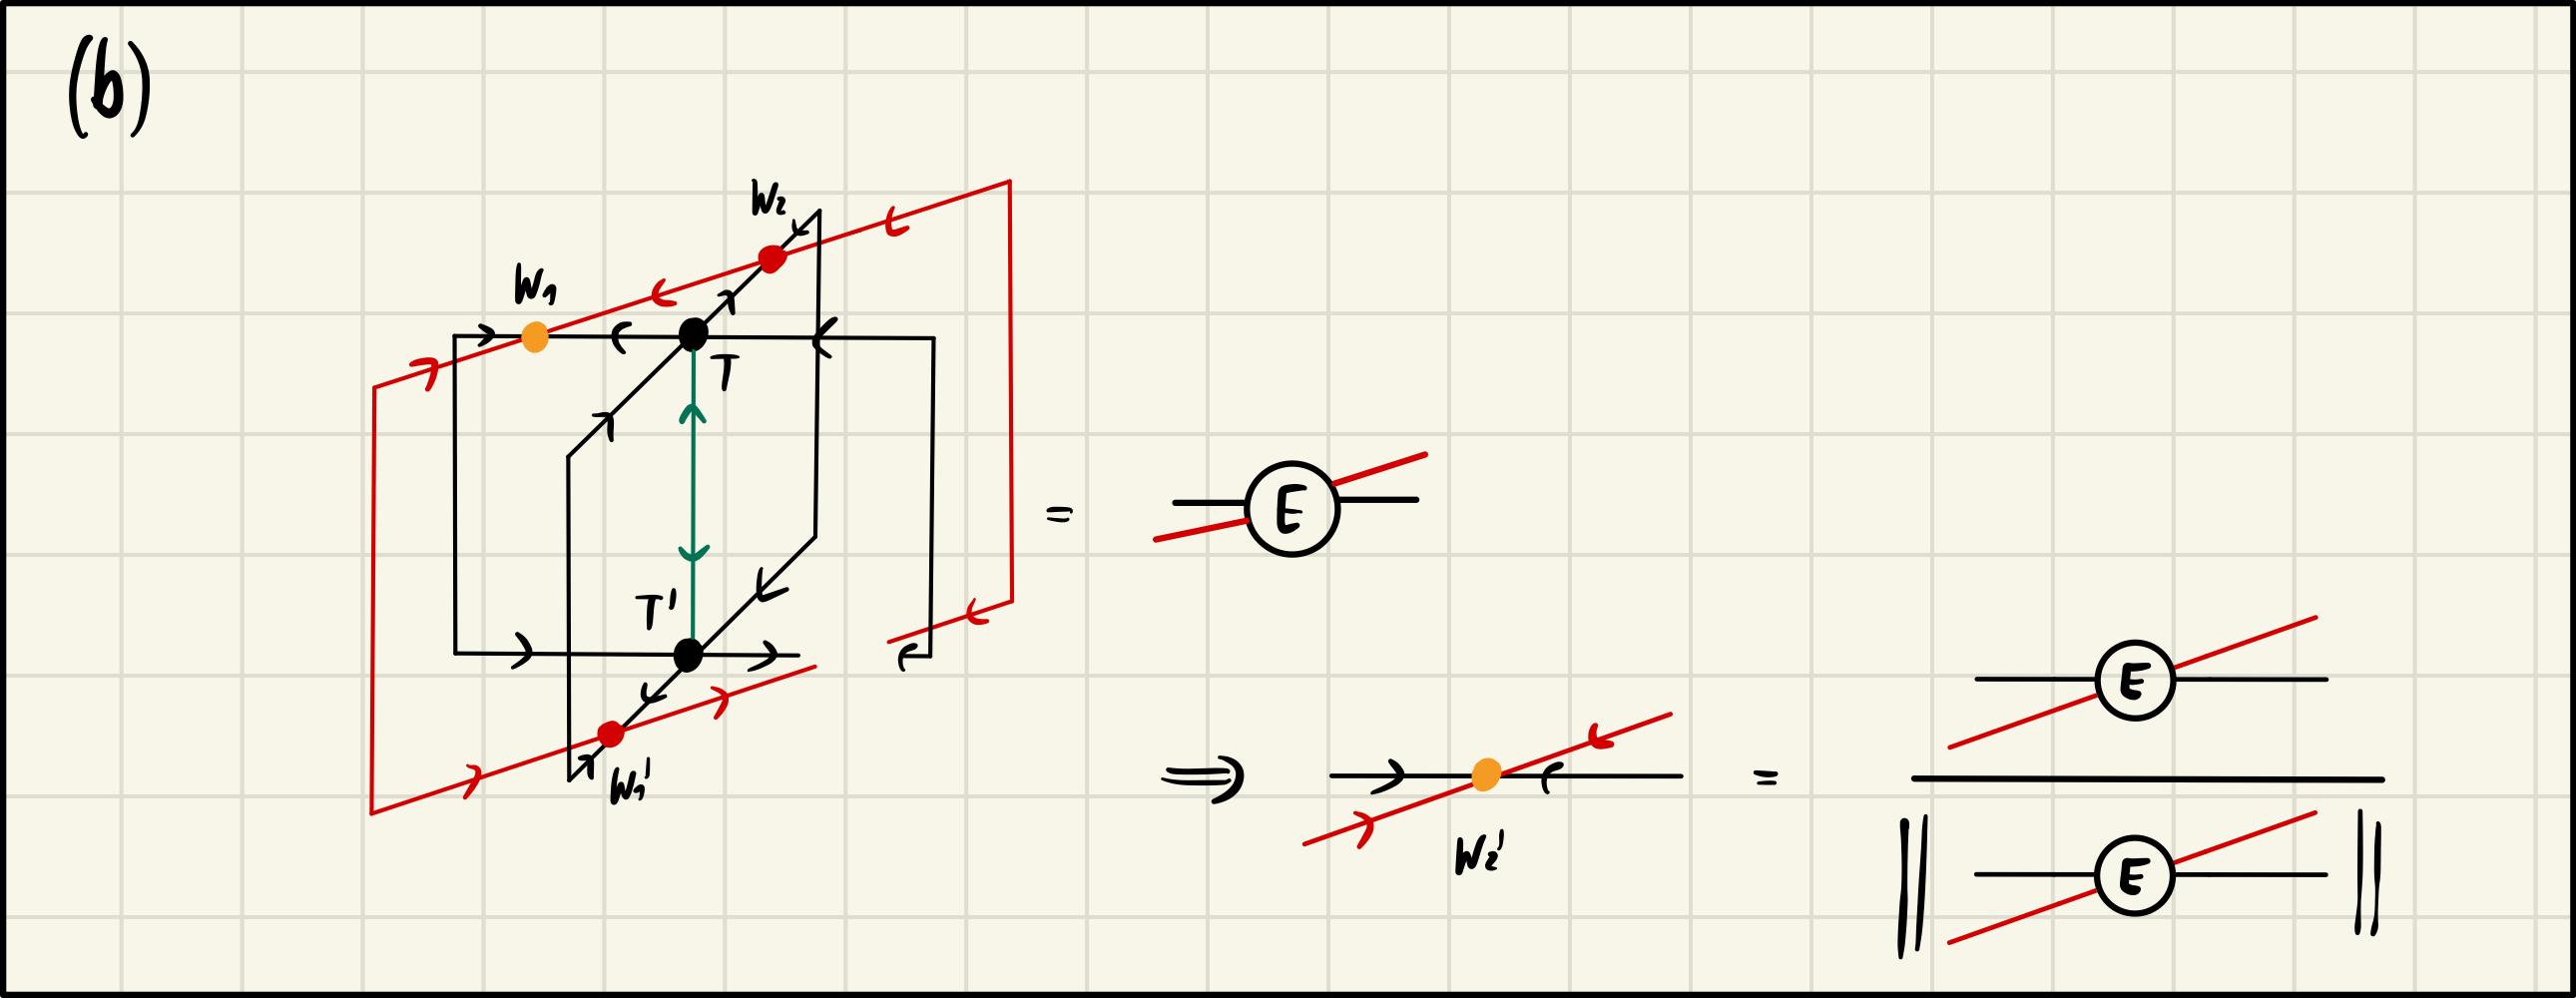
\includegraphics[width=0.6\textwidth]{figures/disoTPS/YB_move_iterate_polar_b.jpeg}
	}
	\subcaptionbox{\label{fig:YB_move_iterate_polar_optimize_W1}}
	{%
		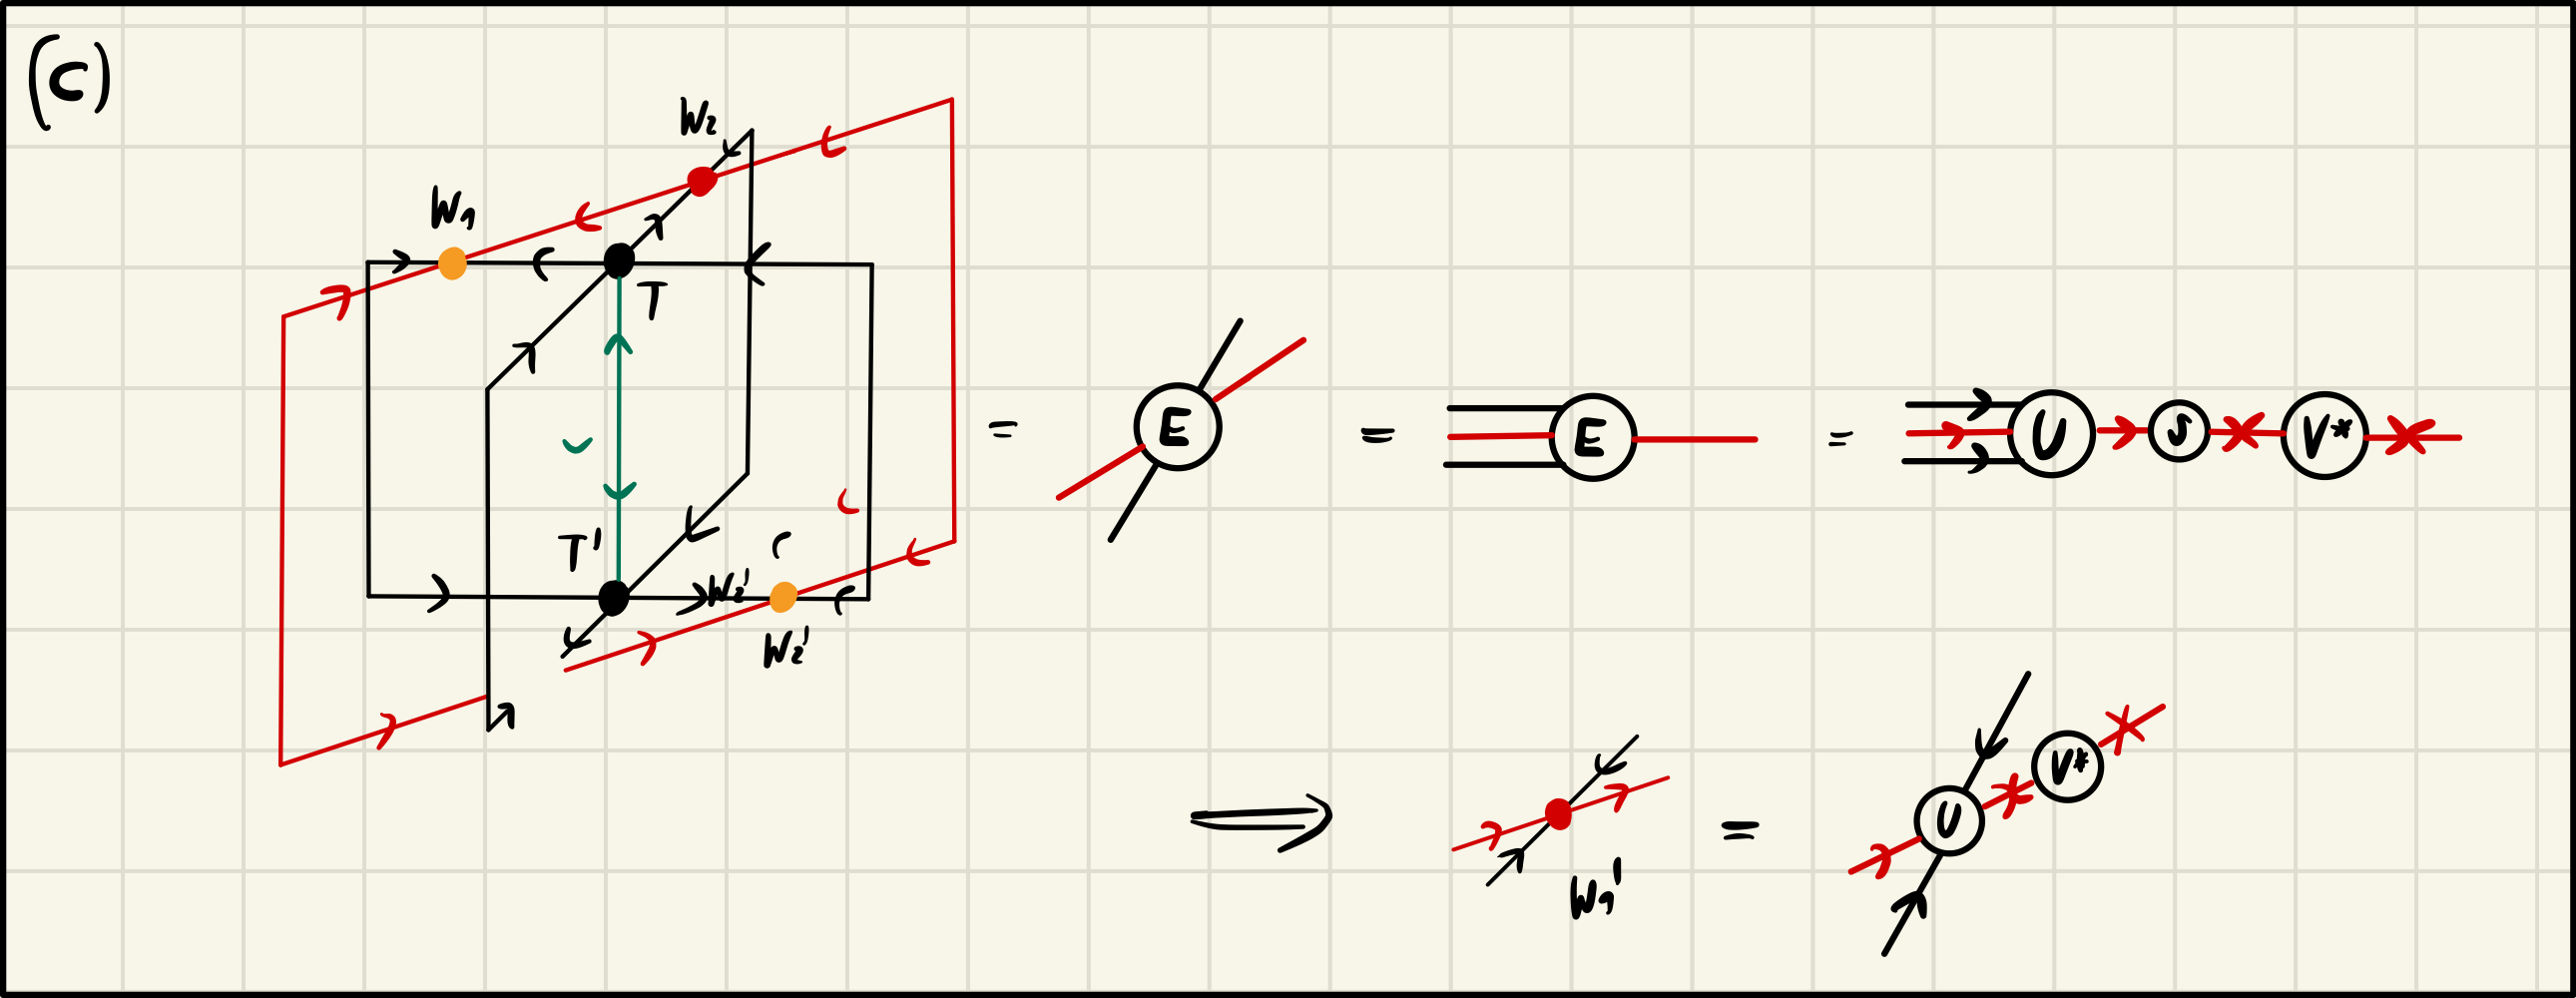
\includegraphics[width=0.6\textwidth]{figures/disoTPS/YB_move_iterate_polar_c.jpeg}
	}
	\subcaptionbox{\label{fig:YB_move_iterate_polar_optimize_T}}
	{%
		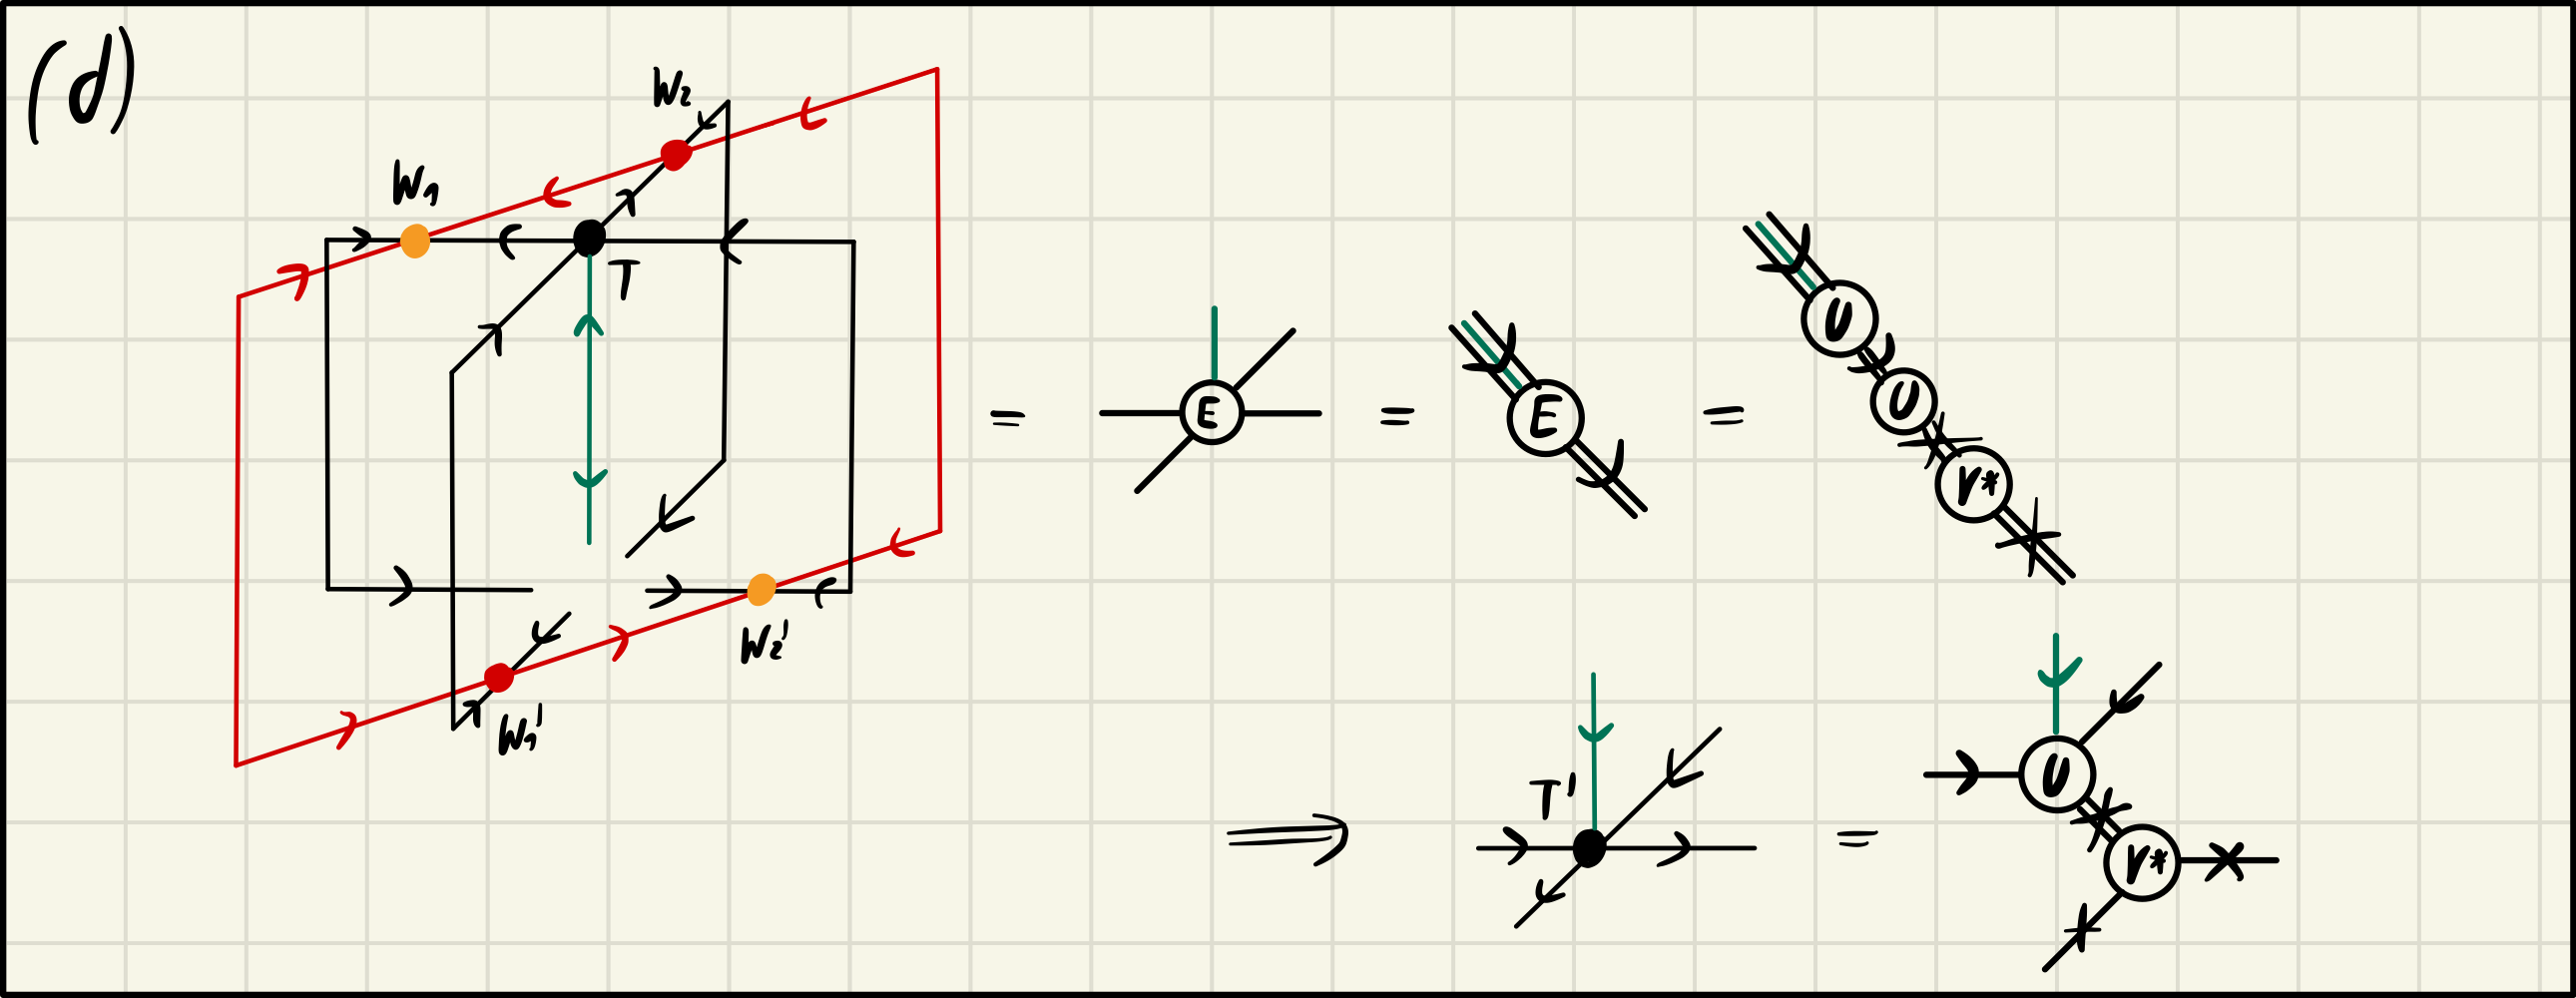
\includegraphics[width=0.6\textwidth]{figures/disoTPS/YB_move_iterate_polar_d.jpeg}
	}
	\caption{(a) The cost function of the optimization problem \eqref{eq:disoTPS_YB_move_alternative_formulation} can be computed as a contraction of only six tensors. (b) To optimize the tensor $W_2^\prime$, all tensors except $W_2^\prime$ are contracted into the environment $E$. The updated tensor is then given as $W_2^\prime = E/\lVert E\rVert$. (c) The tensor $W_1^\prime$ can be updated by contracting all tensors except $W_1^\prime$ into the environment $E$, which is subsequently isometrized using an SVD. (d) The tensor $T^\prime$ can be updated similarly by contracting all tensors except $T^\prime$ into the environment $E$ and isometrizing $E$ using an SVD.}
	\label{fig:YB_move_iterate_polar}
\end{figure}